\subsection*{Предсказание вероятностей}
Прежде чем задавать какие"=либо вопросы касаемо заголовка, давайте рассмотрим более подробно саму классификацию.

Итак, на текущий момент наша модель классификации должна уметь предсказывать конкретный класс для объекта "--- спам письмо или нет, здоров пациент или нет... Но иногда эта информация не является исчерпывающей "--- например, нет прогноза погоды, который однозначно бы предсказывал погоду следующей недели.

Мы привыкли воспринимать прогноз погоды не как \texttt{ground truth} (100\% "=я правда), а как некоторое \textit{достаточно вероятное убеждение}. То есть не факт, что то, что сказали по телевизору, будет в действительности на улице. И тут важно понимать, что сейчас мы рассмотрели модель с \textit{вероятностной точки зрения} "--- модель возвращает не только класс, но и некоторую вероятность, с которой этот объект действительно имеет данный класс.

Давайте рассмотрим более реальный пример "--- пусть задача модели состоит в том, чтобы предсказать, кликнет ли пользователь на рекламный баннер, или нет. При одних и тех же данных (один и тот же баннер, один и тот же сайт и один и тот же пользователь) целевая переменная может варьироваться. Представьте, что обычно Вы пропускаете рекламу, но в какой"=то момент Вам стало настолько нечего делать, что Вы решили поддаться искушению и кликнуть на этот баннер. С точки зрения данных, у одного и того же объекта появилось 2 вхождения: в одном из них вы успешно проигнорировали баннер, а во втором "--- нажали на него.

Именно в таких задачах решает оценивание вероятности, с которой пользователь нажмёт на баннер.

Давайте ближе к сути: мы хотим получить модель $b(x)$, которая будет выдавать значение из интервала $[0, 1]$, а затем мы будем интерпретировать это значение как вероятность положительного класса. То есть, пусть у нас есть часть объектов из выборки, на которых выход модели $b(x) \approx 0.7$. Это означает, что 70\% объектов из этой области действительно должно иметь положительный класс.

\newpage

\subsection*{Логистическая регрессия.}
Так или иначе, мы хотим предсказывать вероятности. Идея заключается в том, что наша модель должна возвращать какое-то значение с интервала $[0, 1]$, и в процессе обучения подгонять эти значения так, чтобы они были как можно ближе к реальным вероятностям. Но сейчас мы умеем пользоваться разве что моделью регрессии:
\[
a(x) = w^Tx
\]
Соответственно, нам нужна какая"=то \textit{осмысленная} функция $f: \mathbb{R} \rightarrow [0, 1]$. Сейчас мы постараемся грамотно её вывести.

Во"=первых скажем, что пусть есть некоторая вероятность события $X$, которая обозначается как $P(X)$. В таком случае, понятие \textit{шанса} определяется как
\[
OR(X) = \frac{P(X)}{1 - P(X)}
\]

Ну например, пусть есть какое"=то событие, вероятность которого $0,8$. В таком случае шанс этого события будут $\frac{ 0,8 } { 0,2 } = \frac{4}{1}$, то есть 4 к 1.

Данная величина может принимать значения в интервале $[0, \infty]$. Для того, чтобы она распространялась на весь $\mathbb{R}$, достаточно просто взять логарифм $\ln$.

В соответствии с правилами логарифмирования, получим 
\[
OR(X) = \exp^{w^Tx}
\]

Таким образом, мы научились из вероятности события получать значение выхода модели. Проблема лишь в том, что нам нужно с точностью наоборот "--- благо проблем с этим возникнуть не должно:
\[
p = \frac{e^{w^Tx}}{1 + e^{w^Tx}} = \frac{1}{1 + e^{-w^Tx}}
\]

Полученную функцию называют \textit{сигмоидой} и обозначают $\sigma(w, x)$. (Обычно говорят, что $z = w^Tx$, и тогда просто $\sigma(z)$).

\begin{figure}[H]
    \centering
    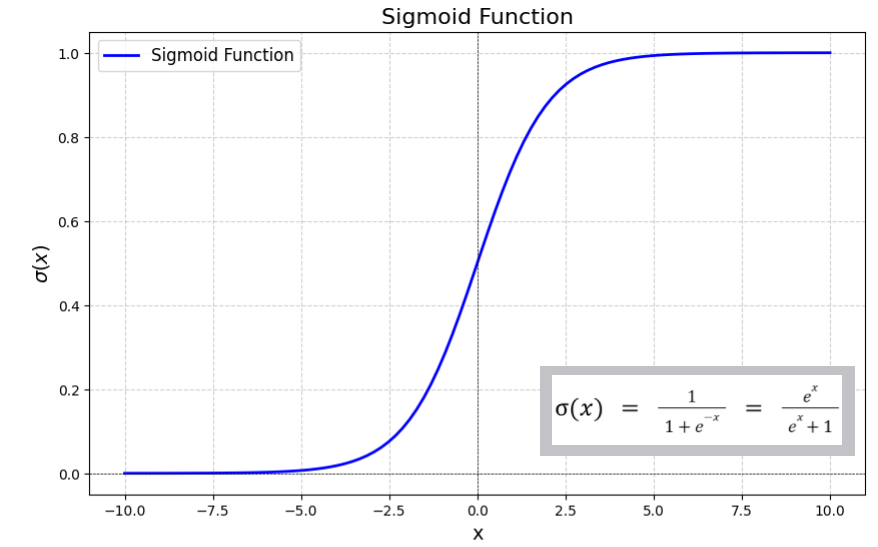
\includegraphics[width=0.9\linewidth]{media/sigmoid.png}
\end{figure}

Ну и по факту, процесс обучения почти готов: берём нашу обычную регрессию, её выходы пропускаем в $\sigma(z)$, получаем какие"=то числа, и процесс обучения сводится к тому, чтобы получать какие"=то вероятности. Нам лишь осталось понять, какую функцию потерь использовать.

\subsection*{Вывод функции потерь для логистической регрессии.}

И тут нам снова придётся откатиться немного назад, в <<истоки>> наших рассуждений. Давайте рассмотрим самый примитивный случай, в котором мы просто будем подбрасывать монетку, и взглянем на эту задачу под другим углом. Наточенный ум при виде монетки может предположить, что мы будем предсказывать вероятность выпадения определённой стороны, но сейчас мы будем заниматься в корни противоположным "--- нам изначально даны все исходы, а наша задача сказать, насколько это \textit{правдоподобно}.

В случае классификации (как и в случае с монеткой), существует всего 2 исхода. И вероятность каждого можно посчитать соответственно как 
\[
p_+ = p;~~~~~~ p_- = 1 - p
\]

Соответственно, вероятность наблюдать именно такие результаты, на самом деле, посчитать не так уж и трудно "--- достаточно перемножить все возможные исходы:
\[
\prod_{i=1}^\ell p^{y_i} (1 - p)^{1 - y_i}
\]
Например, если исход $y_i = 1$, то в конкретном множителе будет лишь $p$, а часть с $(1 - p )^{1 - y_i}$ просто занулится. По такому принципу будет считаться произведение всех таких событий.

Здесь важно понять, что мы хотим, чтобы правдопдобие было как можно больше, т.е. чтобы наблюдаемые нами данные были как можно более реалистичными.

Давайте немного видоизменим формулу:
\begin{enumerate}
    \item Вместо $p$ подставим выход нашей модели, т.к. мы собираемся предсказывать эти самые вероятности;
    \item Внесём логарифм, чтобы вместо произведения было суммирование;
    \item В МО функции потерь привычно \textit{минимизировать}, поэтому поставим отрицание для этой функции;
    \item Вместо возведения в степень введём уже знакомый нам предикат.
\end{enumerate}

Давайте рассмотрим, что получилось:
\[
L(y, z) = - \frac{1}{\ell}\sum_{i=1}^\ell ([y_i = +1]\log b(z) + [y_i = -1](1 - \log b(z)))
\]

В действительности, это и есть функция потерь \texttt{LogLoss}, но для полной красоты давайте подставим $b(z) = \sigma(\langle w,x\rangle + b)$. Тогда получим заветное
\[
-\frac{1}{\ell}\sum_{i=1}^\ell \log(1 + \exp^{-M_i}) \rightarrow \min_w
\]

Получили процесс обучения логистической регрессии.